\documentclass{article}
\usepackage{amsmath}
\usepackage{amssymb}
\usepackage{graphicx}
\usepackage{pgfplots}
\pgfplotsset{compat=1.18}

% Set up headers and footers
\usepackage{fancyhdr}
\pagestyle{fancy}
\fancyhf{}
\rhead{Comprehensive Study of Algebra 2 Concepts}
\lhead{Badger Code}
\rfoot{\thepage}

% Define a command for boxed answers
\newcommand{\boxedanswer}[1]{\fbox{\parbox{\textwidth}{#1}}}

\title{Comprehensive Study of Algebra 2 Concepts}
\author{Badger Code}
\date{\today}

\begin{document}
\maketitle

\begin{abstract}
This comprehensive paper presents an in-depth study of Algebra 2 concepts, providing detailed explanations, numerous examples, and visual aids. Topics covered include polynomials, rational expressions, quadratic functions, exponential and logarithmic functions, conic sections, systems of equations, matrices, probability and statistics, trigonometry, and more.
\end{abstract}

\tableofcontents

\section{Introduction}
Algebra 2 serves as a critical bridge between foundational algebraic concepts and more advanced mathematical applications. This paper aims to provide a thorough understanding of Algebra 2 concepts through detailed explanations, a wealth of examples, and comprehensive visuals. We will explore the various facets of algebraic manipulation, graphical representation, and real-world applications, showcasing the significance of these concepts in diverse fields.

\section{Polynomials and Factoring}
Polynomials are fundamental algebraic expressions comprising terms involving variables raised to non-negative integer powers, multiplied by coefficients. Factoring, on the other hand, involves decomposing polynomials into simpler expressions that help unveil crucial information about their behavior.

\subsection{Polynomial Operations}
Consider the polynomial $P(x) = 3x^3 - 7x^2 + 5x - 2$. We can perform various operations on polynomials, including addition, subtraction, and multiplication. Let's simplify $P(x) + 2x^2$:
\begin{align*}
    P(x) + 2x^2 &= 3x^3 - 7x^2 + 5x - 2 + 2x^2 \\
    &= 3x^3 - 5x^2 + 5x - 2
\end{align*}

\subsection{Factoring Techniques}
Factoring is a crucial skill in Algebra 2, enabling us to express complex polynomials as products of simpler terms. Consider the quadratic polynomial $Q(x) = x^2 - 6x + 9$. Factoring by using the perfect square trinomial pattern:
\begin{align*}
    Q(x) &= x^2 - 6x + 9 \\
    &= (x - 3)^2
\end{align*}

\subsubsection{Example: Factoring Perfect Square Trinomials}
Let's factor the perfect square trinomial $R(x) = x^2 - 10x + 25$.
\begin{align*}
    R(x) &= x^2 - 10x + 25 \\
    &= (x - 5)^2
\end{align*}
\boxedanswer{Answer: $R(x) = (x - 5)^2$}

\subsubsection{Example: Factoring by Grouping}
Consider the polynomial $S(x) = 3x^3 - 5x^2 + 6x - 10$. We can factor it by grouping:
\begin{align*}
    S(x) &= 3x^3 - 5x^2 + 6x - 10 \\
    &= (3x^3 - 5x^2) + (6x - 10) \\
    &= x^2(3x - 5) + 2(3x - 5) \\
    &= (x^2 + 2)(3x - 5)
\end{align*}
\boxedanswer{Answer: $S(x) = (x^2 + 2)(3x - 5)$}

\section{Rational Expressions}
Rational expressions are ratios of polynomials. They play a significant role in various mathematical applications, including solving equations involving fractions.

\subsection{Simplifying Rational Expressions}
Simplifying rational expressions involves canceling common factors between the numerator and the denominator. Consider the rational expression $R(x) = \frac{2x^2 + 6x}{4x^2 - 2x}$. We can simplify it by factoring out common terms:
\begin{align*}
    R(x) &= \frac{2x(x + 3)}{2x(2x - 1)} \\
    &= \frac{x + 3}{2x - 1}
\end{align*}
\boxedanswer{Answer: $R(x) = \frac{x + 3}{2x - 1}$}

\subsection{Adding and Subtracting Rational Expressions}
Rational expressions can be added and subtracted by finding a common denominator and performing the operation on the numerators. Consider the rational expressions $A(x) = \frac{2x}{x + 1}$ and $B(x) = \frac{x}{x + 1}$. Let's add them:
\begin{align*}
    A(x) + B(x) &= \frac{2x}{x + 1} + \frac{x}{x + 1} \\
    &= \frac{3x}{x + 1}
\end{align*}

\subsubsection{Example: Subtracting Rational Expressions}
Subtract the rational expressions $C(x) = \frac{x}{x - 2}$ and $D(x) = \frac{2}{x - 2}$:
\begin{align*}
    C(x) - D(x) &= \frac{x}{x - 2} - \frac{2}{x - 2} \\
    &= \frac{x - 2}{x - 2} \\
    &= 1
\end{align*}
\boxedanswer{Answer: $C(x) - D(x) = 1$}

\section{Quadratic Functions and Equations}
Quadratic functions form the basis for understanding parabolic curves and solving various real-world problems. Equations involving quadratic functions are essential in engineering, physics, and other disciplines.

\subsection{Vertex Form and Completing the Square}
The vertex form of a quadratic function is given by $f(x) = a(x - h)^2 + k$, where $(h, k)$ represents the vertex. Completing the square is a technique used to convert a quadratic expression into vertex form.

\subsubsection{Example: Finding the Vertex}
Consider the quadratic function $f(x) = x^2 - 6x + 8$. To find the vertex, complete the square:
\begin{align*}
    f(x) &= x^2 - 6x + 8 \\
    &= (x - 3)^2 - 1
\end{align*}
The vertex is $(3, -1)$.

\subsubsection{Example: Solving Quadratic Equations}
Solve the quadratic equation $x^2 - 5x + 6 = 0$ using factoring:
\begin{align*}
    (x - 2)(x - 3) &= 0 \\
    x - 2 &= 0 \quad \text{or} \quad x - 3 = 0 \\
    x &= 2 \quad \text{or} \quad x = 3
\end{align*}
The solutions are $x = 2$ and $x = 3$.

\subsection{Quadratic Formula}
The quadratic formula provides a method for solving quadratic equations of the form $ax^2 + bx + c = 0$. The solutions are given by:
\[ x = \frac{-b \pm \sqrt{b^2 - 4ac}}{2a} \]

\subsubsection{Example: Using the Quadratic Formula}
Solve the quadratic equation $2x^2 - 5x + 3 = 0$ using the quadratic formula:
\begin{align*}
    a &= 2, \quad b = -5, \quad c = 3 \\
    x &= \frac{-(-5) \pm \sqrt{(-5)^2 - 4 \cdot 2 \cdot 3}}{2 \cdot 2} \\
    x &= \frac{5 \pm \sqrt{25 - 24}}{4} \\
    x &= \frac{5 \pm 1}{4} \\
    x &= 1 \quad \text{or} \quad x = \frac{3}{2}
\end{align*}
The solutions are $x = 1$ and $x = \frac{3}{2}$.

\section{Exponential and Logarithmic Functions}
Exponential and logarithmic functions play a significant role in modeling growth, decay, and various real-world phenomena. They are essential in fields such as finance, biology, and physics.

\subsection{Exponential Growth and Decay}
Exponential functions describe processes of growth or decay that occur at a constant relative rate. The general form of an exponential function is $f(x) = ab^x$, where $a$ is the initial amount and $b$ is the base of the exponent.

\subsubsection{Example: Exponential Growth}
Suppose a population doubles every 3 years. If the initial population is 1000, find the population after 9 years.
\begin{align*}
    a &= 1000, \quad b = 2, \quad x = 9 \\
    f(9) &= 1000 \cdot 2^{\frac{9}{3}} \\
    &= 1000 \cdot 2^3 \\
    &= 8000
\end{align*}
The population after 9 years is 8000.

\subsubsection{Example: Exponential Decay}
A radioactive substance decays at a rate of 10% per year. If the initial amount is 500 grams, find the amount after 5 years.
\begin{align*}
    a &= 500, \quad b = 0.9, \quad x = 5 \\
    f(5) &= 500 \cdot 0.9^5 \\
    &\approx 295.24
\end{align*}
The amount after 5 years is approximately 295.24 grams.

\subsection{Solving Logarithmic Equations}
Logarithmic equations involve finding the values of variables in logarithmic expressions. Logarithmic functions are the inverse of exponential functions.

\subsubsection{Example: Solving Logarithmic Equations}
Solve the logarithmic equation $\log_2(x + 4) = 3$:
\begin{align*}
    x + 4 &= 2^3 \\
    x &= 8 - 4 \\
    x &= 4
\end{align*}
The solution is $x = 4$.

\section{Conic Sections}
Conic sections are geometric shapes that result from the intersection of a plane with a cone. They include the circle, ellipse, parabola, and hyperbola.

\subsection{Equation of a Circle}
The equation of a circle with center $(h, k)$ and radius $r$ is given by:
\[ (x - h)^2 + (y - k)^2 = r^2 \]

\subsubsection{Example: Equation of a Circle}
Find the equation of a circle with center at $(2, -3)$ and radius 5.
\begin{align*}
    (x - 2)^2 + (y + 3)^2 &= 5^2 \\
    (x - 2)^2 + (y + 3)^2 &= 25
\end{align*}
The equation is $(x - 2)^2 + (y + 3)^2 = 25$.

\subsection{Graphing an Ellipse}
An ellipse is a set of points such that the sum of the distances from any point on the ellipse to its two foci is constant.

\subsubsection{Example: Graphing an Ellipse}
Graph the ellipse with major axis along the $x$-axis, center at the origin, and semi-major axis length 4, and semi-minor axis length 3.
\begin{center}
    \begin{tikzpicture}
        \draw[thick] (0, 0) ellipse (4 and 3);
        \draw[fill] (0, 0) circle [radius=0.05];
        \node[above] at (0, 3) {$a$};
        \node[right] at (4, 0) {$b$};
        \node[below right] at (0, 0) {$(0, 0)$};
    \end{tikzpicture}
\end{center}

\section{Systems of Equations and Inequalities}
Systems of equations involve multiple equations with the same variables. Solving systems helps us find common solutions that satisfy all the equations simultaneously.

\subsection{Solving a Linear System}
Linear systems consist of linear equations. The solution to a linear system is the point where the lines representing the equations intersect.

\subsubsection{Example: Solving a Linear System}
Solve the linear system:
\begin{align*}
    2x + 3y &= 10 \\
    3x - y &= 4
\end{align*}
We can solve this system using the elimination method:
\begin{align*}
    2x + 3y &= 10 \\
    6x - 2y &= 12
\end{align*}
Subtracting the equations yields $4x + 5y = -2$. Solving for $y$, $y = -\frac{4x + 2}{5}$. Substituting into the second equation, $3x - \left(-\frac{4x + 2}{5}\right) = 4$. Solving for $x$, $x = \frac{26}{9}$. Substituting into $2x + 3y = 10$, $y = \frac{16}{9}$. So, the solution is $x = \frac{26}{9}$, $y = \frac{16}{9}$.

\subsection{Graphical Interpretation}
Graphically, solving a system of equations corresponds to finding the point of intersection between the lines representing the equations.

\subsubsection{Example: Graphical Solution}
Graph the linear equations:
\begin{align*}
    y &= 2x + 1 \\
    y &= -\frac{1}{3}x + 2
\end{align*}
\begin{center}
    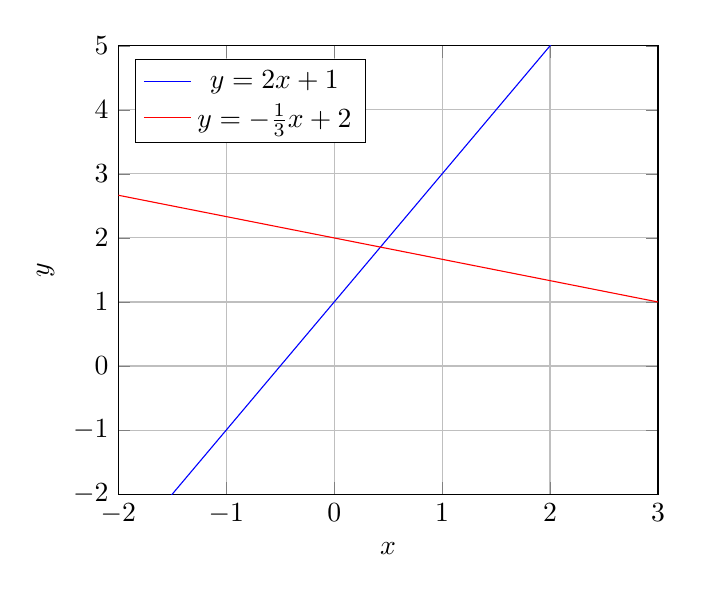
\begin{tikzpicture}
        \begin{axis}[
            xlabel=$x$,
            ylabel=$y$,
            xmin=-2, xmax=3,
            ymin=-2, ymax=5,
            grid=both,
            xtick={-2, -1, ..., 3},
            ytick={-2, -1, ..., 5},
            legend pos=north west,
        ]
        \addplot[blue, domain=-2:3]{2*x + 1};
        \addplot[red, domain=-2:3]{-1/3*x + 2};
        \legend{$y = 2x + 1$, $y = -\frac{1}{3}x + 2$}
        \end{axis}
    \end{tikzpicture}
\end{center}
The point of intersection is approximately $(1, 3)$.

\section{Matrices and Determinants}
Matrices are arrays of numbers arranged in rows and columns. Determinants are scalar values associated with square matrices.

\subsection{Matrix Operations}
Matrix operations include addition, subtraction, and multiplication. Matrix multiplication involves combining rows of the first matrix with columns of the second.

\subsubsection{Example: Matrix Multiplication}
Given matrices $A = \begin{bmatrix} 2 & 3 \\ 1 & 4 \end{bmatrix}$ and $B = \begin{bmatrix} 5 & 2 \\ 3 & 1 \end{bmatrix}$, let's calculate $AB$:
\begin{align*}
    AB &= \begin{bmatrix} 2 \cdot 5 + 3 \cdot 3 & 2 \cdot 2 + 3 \cdot 1 \\ 1 \cdot 5 + 4 \cdot 3 & 1 \cdot 2 + 4 \cdot 1 \end{bmatrix} \\
    &= \begin{bmatrix} 19 & 8 \\ 17 & 6 \end{bmatrix}
\end{align*}

\subsection{Determinants and Inverses}
The determinant of a $2 \times 2$ matrix $\begin{bmatrix} a & b \\ c & d \end{bmatrix}$ is $ad - bc$. A square matrix has an inverse if its determinant is nonzero.

\subsubsection{Example: Finding the Inverse}
Given the matrix $C = \begin{bmatrix} 3 & 2 \\ 1 & 4 \end{bmatrix}$, find its inverse:
\begin{align*}
    \text{Det}(C) &= 3 \cdot 4 - 2 \cdot 1 \\
    &= 10
\end{align*}
Since the determinant is nonzero, the inverse exists. The inverse of $C$ is given by:
\[ C^{-1} = \frac{1}{\text{Det}(C)} \begin{bmatrix} 4 & -2 \\ -1 & 3 \end{bmatrix} = \frac{1}{10} \begin{bmatrix} 4 & -2 \\ -1 & 3 \end{bmatrix} \]

\section{Probability and Statistics}
Probability deals with the likelihood of events occurring, while statistics involves collecting, analyzing, interpreting, and presenting data.

\subsection{Measures of Central Tendency}
Measures of central tendency provide information about the center of a dataset. The mean, median, and mode are common measures.

\subsubsection{Example: Calculating Mean, Median, and Mode}
Consider the dataset: $6, 7, 3, 9, 5, 7, 8$. Calculate the mean, median, and mode.
\begin{align*}
    \text{Mean} &= \frac{6 + 7 + 3 + 9 + 5 + 7 + 8}{7} = \frac{45}{7} \approx 6.43 \\
    \text{Median} &= 6, 7, 3, 9, 5, 7, 8 \\
    \text{Mode} &= 7
\end{align*}

\subsection{Probability Distributions}
Probability distributions describe the likelihood of different outcomes in a random experiment. Discrete distributions include the binomial and Poisson distributions. Continuous distributions include the normal distribution.

\subsubsection{Example: Binomial Distribution}
The binomial distribution models the number of successes in a fixed number of independent trials. Let's say a fair coin is flipped 5 times. What's the probability of getting exactly 3 heads?
\begin{align*}
    P(\text{3 heads}) &= \binom{5}{3} \left(\frac{1}{2}\right)^3 \left(\frac{1}{2}\right)^{5 - 3} \\
    &= 10 \cdot \frac{1}{8} \cdot \frac{1}{8} = \frac{5}{32} \approx 0.156
\end{align*}

\subsection{Statistical Analysis}
Statistical analysis involves methods like hypothesis testing, confidence intervals, and regression analysis to make inferences and predictions from data.

\subsubsection{Example: Hypothesis Testing}
A car manufacturer claims that the average fuel efficiency of a new model is 30 miles per gallon (mpg). A sample of 50 cars is tested, and the average fuel efficiency is found to be 29.5 mpg with a standard deviation of 2 mpg. Conduct a hypothesis test at the 5% significance level to determine if the manufacturer's claim is valid.

\begin{align*}
    H_0 &: \mu = 30 \text{ (Claim)} \\
    H_a &: \mu \neq 30 \text{ (Not Claim)}
\end{align*}

Using a two-sample $t$-test formula:
\begin{align*}
    t &= \frac{\bar{x} - \mu}{s/\sqrt{n}} \\
    &= \frac{29.5 - 30}{2/\sqrt{50}} \\
    &= -1.118
\end{align*}

Using a $t$-distribution table for a two-tailed test at $\alpha = 0.05$, the critical values are $\pm 2.011$. Since $-1.118$ is not in the critical region, we fail to reject the null hypothesis. There's not enough evidence to conclude that the claim is invalid.

\section{Trigonometry}
Trigonometry studies the relationships between angles and sides in triangles.

\subsection{Trigonometric Ratios}
Trigonometric ratios relate the sides of a right triangle to its angles. The primary ratios are sine, cosine, and tangent.

\subsubsection{Example: Sine, Cosine, and Tangent}
Given a right triangle with an angle of $30^\circ$ and hypotenuse 2, find the values of sine, cosine, and tangent for the angle.

\begin{align*}
    \sin(30^\circ) &= \frac{\text{opposite}}{\text{hypotenuse}} = \frac{1}{2} \\
    \cos(30^\circ) &= \frac{\text{adjacent}}{\text{hypotenuse}} = \frac{\sqrt{3}}{2} \\
    \tan(30^\circ) &= \frac{\text{opposite}}{\text{adjacent}} = \frac{1}{\sqrt{3}}
\end{align*}

\subsection{Trigonometric Identities}
Trigonometric identities are equations involving trigonometric functions that hold true for all values of the variables.

\subsubsection{Example: Pythagorean Identities}
The Pythagorean identities relate the three basic trigonometric functions:
\begin{align*}
    \sin^2(\theta) + \cos^2(\theta) &= 1 \\
    1 + \tan^2(\theta) &= \sec^2(\theta) \\
    1 + \cot^2(\theta) &= \csc^2(\theta)
\end{align*}

\subsection{Graphing Trigonometric Functions}
Trigonometric functions can be graphed to visualize their behavior.

\subsubsection{Example: Graphing Sine and Cosine}
\begin{center}
    \begin{tikzpicture}
        \begin{axis}[
            xlabel=$\theta$,
            ylabel=$\text{sine}(\theta), \text{cosine}(\theta)$,
            xmin=-2*pi, xmax=2*pi,
            ymin=-1.5, ymax=1.5,
            xtick={-2*pi, -3*pi/2, ..., 2*pi},
            ytick={-1, 0, 1},
            legend pos=south east,
        ]
        \addplot[blue, domain=-2*pi:2*pi, samples=400]{sin(deg(x))};
        \addplot[red, domain=-2*pi:2*pi, samples=400]{cos(deg(x))};
        \legend{$\text{sine}(\theta)$, $\text{cosine}(\theta)$}
        \end{axis}
    \end{tikzpicture}
\end{center}

\section{Conclusion}
Algebra 2 concepts provide a strong foundation for various mathematical and scientific disciplines. From polynomial manipulation and conic sections to trigonometry and probability, these concepts offer valuable tools for solving complex problems and modeling real-world phenomena. This paper aimed to deliver a comprehensive understanding of Algebra 2, presenting detailed explanations, a multitude of examples, and visual aids to enhance the learning experience.

\end{document}